\documentclass[12pt,a4paper]{article}

% ─── Page Layout ───────────────────────────────────────────────────────────────
\usepackage[a4paper, margin=0.8in, headheight=14pt]{geometry}

% ─── Fonts (XeLaTeX) ───────────────────────────────────────────────────────────
\usepackage{fontspec}
\usepackage{unicode-math}
\setmainfont{TeX Gyre Pagella}
\setmonofont[Scale=0.88]{TeX Gyre Cursor}
\setmathfont{Latin Modern Math}

% ─── Packages ──────────────────────────────────────────────────────────────────
\usepackage{xcolor}
\usepackage{colortbl}
\usepackage{titlesec}
\usepackage{enumitem}
\usepackage{tabularx}
\usepackage{booktabs}
\usepackage{array}
\usepackage{amsmath}
\usepackage{tikz}
\usetikzlibrary{shapes.geometric, arrows.meta, positioning, calc, fit, decorations.pathreplacing}
\usepackage{tcolorbox}
\tcbuselibrary{skins, breakable}
\usepackage{hyperref}
\usepackage{fancyhdr}
\usepackage{graphicx}
\usepackage{microtype}
\hyphenpenalty=10000
\exhyphenpenalty=10000
\sloppy
\usepackage{caption}
\usepackage{setspace}
\usepackage{multirow}
\usepackage{tocloft}

% ─── Q&A helper ────────────────────────────────────────────────────────────────
\newcommand{\Q}[1]{\textbf{#1}\par\noindent\ignorespaces}

% ─── Colour Palette ────────────────────────────────────────────────────────────
\definecolor{myred}{RGB}{196,30,58}
\definecolor{mydark}{RGB}{30,30,50}
\definecolor{mygreen}{RGB}{14,120,80}
\definecolor{myteal}{RGB}{0,130,140}
\definecolor{myamber}{RGB}{180,100,0}
\definecolor{mypurple}{RGB}{100,30,160}
\definecolor{mygray}{RGB}{246,247,249}
\definecolor{mgframe}{RGB}{180,185,200}
\definecolor{watermark}{RGB}{145,150,170}
\definecolor{hdrred}{RGB}{250,232,235}
\definecolor{hdrgreen}{RGB}{220,244,233}
\definecolor{hdrteal}{RGB}{220,242,244}
\definecolor{hdramber}{RGB}{253,242,215}
\definecolor{hdrpurple}{RGB}{238,228,255}
\definecolor{hdrgray}{RGB}{238,240,245}
\definecolor{rowalt}{RGB}{250,251,253}

% ─── Section Formatting ────────────────────────────────────────────────────────
\titleformat{\section}
  {\large\bfseries\color{myred}}{\thesection.}{0.5em}{}
  [\vspace{1pt}{\color{myred}\rule{\linewidth}{0.8pt}}]
\titleformat{\subsection}
  {\normalsize\bfseries\color{myteal}}{\thesubsection}{0.5em}{}
\titlespacing*{\section}{0pt}{18pt}{7pt}
\titlespacing*{\subsection}{0pt}{11pt}{4pt}

% ─── Paragraph ─────────────────────────────────────────────────────────────────
\setlength{\parindent}{0pt}
\setlength{\parskip}{4pt}

% ─── TOC Styling ───────────────────────────────────────────────────────────────
\renewcommand{\cfttoctitlefont}{\large\bfseries\color{myred}}
\renewcommand{\cftaftertoctitle}{\par\noindent{\color{myred}\rule{\linewidth}{0.8pt}}}
\setlength{\cftbeforetoctitleskip}{0pt}
\setlength{\cftaftertoctitleskip}{6pt}
\renewcommand{\cftsecfont}{\normalsize\bfseries\color{mydark}}
\renewcommand{\cftsecpagefont}{\normalsize\bfseries\color{mydark}}
\renewcommand{\cftsecleader}{\cftdotfill{\cftdotsep}}
\setlength{\cftbeforesecskip}{7pt}
\renewcommand{\cftsubsecfont}{\small\color{mydark}}
\renewcommand{\cftsubsecpagefont}{\small\color{mydark}}
\setlength{\cftbeforesubsecskip}{3pt}
\setlength{\cftsubsecindent}{1.4em}

% ─── Table helpers ─────────────────────────────────────────────────────────────
\renewcommand{\arraystretch}{1.45}
\setlength{\tabcolsep}{6pt}
\arrayrulecolor{mydark}
\newcolumntype{B}[1]{>{\small\bfseries\raggedright\arraybackslash}m{#1}}
\newcolumntype{C}[1]{>{\centering\arraybackslash}m{#1}}
\newcolumntype{Y}{>{\small\raggedright\arraybackslash}X}
\renewcommand{\tabularxcolumn}[1]{m{#1}}

% ─── Header / Footer ───────────────────────────────────────────────────────────
\pagestyle{fancy}
\fancyhf{}
\fancyhead[L]{\small\color{myred}\textbf{OE-EC803C}\;\color{mydark}--- Cyber Security}
\fancyhead[R]{\small\color{myteal}\textbf{Module 4 Notes}}
\fancyfoot[C]{\small\color{mydark}\thepage}
\fancyfoot[R]{\small\color{watermark}\textit{\copyright\ Biraj Sarkar}}
\renewcommand{\headrulewidth}{0.5pt}
\renewcommand{\footrulewidth}{0.3pt}

% ─── Hyperref ──────────────────────────────────────────────────────────────────
\hypersetup{
  colorlinks=true, linkcolor=myteal, urlcolor=myteal,
  pdfauthor={Biraj Sarkar},
  pdftitle={OE-EC803C --- Module 4 Notes}
}

% ─── tcolorbox styles ──────────────────────────────────────────────────────────
\tcbset{
  tikzbox/.style={
    colback=mygray, colframe=mgframe, boxrule=0.6pt, arc=4pt,
    left=8pt, right=8pt, top=6pt, bottom=6pt,
    colbacktitle=mgframe, coltitle=mydark,
    fonttitle=\small\bfseries
  },
  defbox/.style={
    colback=hdrgreen, colframe=mygreen, boxrule=0.8pt, arc=4pt,
    left=9pt, right=9pt, top=6pt, bottom=6pt,
    colbacktitle=mygreen, coltitle=white,
    fonttitle=\small\bfseries
  },
  formulabox/.style={
    colback=hdrteal, colframe=myteal, boxrule=0.8pt, arc=4pt,
    left=9pt, right=9pt, top=7pt, bottom=7pt,
    colbacktitle=myteal, coltitle=white,
    fonttitle=\small\bfseries
  },
  examplebox/.style={
    colback=hdramber, colframe=myamber, boxrule=0.8pt, arc=4pt,
    left=9pt, right=9pt, top=6pt, bottom=6pt,
    colbacktitle=myamber, coltitle=white,
    fonttitle=\small\bfseries
  },
  masonbox/.style={
    colback=hdrpurple, colframe=mypurple, boxrule=0.8pt, arc=4pt,
    left=9pt, right=9pt, top=6pt, bottom=6pt,
    colbacktitle=mypurple, coltitle=white,
    fonttitle=\small\bfseries
  },
  exambox/.style={
    colback=hdrpurple, colframe=mypurple, boxrule=1pt, arc=5pt,
    left=10pt, right=10pt, top=8pt, bottom=8pt,
    colbacktitle=mypurple, coltitle=white, fonttitle=\bfseries,
    breakable, title after break={\textbf{Frequently Asked / Viva Questions (contd.)}}
  }
}
\tcbset{breakable}

% ─── TikZ styles ───────────────────────────────────────────────────────────────
\tikzset{
  block/.style={rectangle, draw=myteal, fill=hdrteal,
    text width=2.2cm, align=center, minimum height=0.9cm,
    font=\small, rounded corners=3pt, line width=0.7pt},
  redblock/.style={rectangle, draw=myred, fill=hdrred,
    text width=2.2cm, align=center, minimum height=0.9cm,
    font=\small, rounded corners=3pt, line width=0.7pt},
  arrow/.style={-Stealth, thick, color=mydark},
  redarrow/.style={-Stealth, thick, color=myred},
  line/.style={thick, color=mydark}
}

\begin{document}

% ═══════════════════════════════════════════════════════════════════════════════
% TITLE BLOCK
% ═══════════════════════════════════════════════════════════════════════════════
\begin{center}
  \hfill \textit{Exam-Ready Short Notes} \\
  \vspace{6pt}
  {\LARGE\bfseries\color{myred} OE-EC803C --- Cyber Security}\\[5pt]
  {\normalsize\color{mydark} Semester VIII \quad$\bullet$\quad 3L:0T:0P \quad$\bullet$\quad 3 Credits}\\[3pt]
  {\normalsize\color{myteal}\textbf{Module 4: Cyber Infrastructure Issues \& International Relations}}\\[3pt]
  {\small\color{mydark} CGEC \;$|$\; B.Tech ECE (2023--27) \;$|$\; \textit{Biraj Sarkar}}
\end{center}
\vspace{2pt}
\noindent{\color{myred}\rule{\linewidth}{1.5pt}}
\vspace{2pt}

\hypersetup{linkcolor=mydark}
\tableofcontents
\hypersetup{linkcolor=myteal}
\newpage

% ===============================================================================
\section{Critical Infrastructure Protection (CIP)}
% ===============================================================================

\begin{tcolorbox}[defbox, title={\textbf{Definition: Critical National Infrastructure (CNI)}}]
\textbf{Critical National Infrastructure (CNI)} encompasses physical and digital systems so vital to a sovereign nation that their disruption would severely paralyze national security, economic stability, public health, or safety.
\end{tcolorbox}

\subsection{Key Sector Threat Profiles and Vulnerabilities}
{\renewcommand{\arraystretch}{1.45}%
\begin{tabularx}{\linewidth}{|B{3.5cm}|Y|Y|}
\hline
\textbf{Sector} & \textbf{Target Systems} & \textbf{Critical Threat Vectors} \\
\hline
Banking \& Finance & SWIFT terminals, Core Banking, Payment Gateways. & Fraudulent wire transfers, ransomware, insider threats. \\
\hline
Healthcare & Electronic Health Records (EHR), IoMT Medical Devices. & Ransomware locking ICU systems, unencrypted patient PII. \\
\hline
Energy \& Power Grid & SCADA networks, Substation PLCs, Smart Meters. & State-sponsored sabotage, air-gap USB malware. \\
\hline
\end{tabularx}}

% ===============================================================================
\section{Economics, Finance, Banking \& Healthcare Security}
% ===============================================================================

\subsection{Economics of Cyber Security}
Cybersecurity is fundamentally an economic problem where threat actors exploit asymmetric costs:
\begin{itemize}[leftmargin=*, itemsep=3pt]
  \item \textbf{Asymmetric Cost Advantage:} Attackers require minimal capital investment to launch automated global exploits, whereas defenders incur high continuous operational costs to protect vast attack surfaces.
  \item \textbf{Return on Security Investment (ROSI):} Financial metric evaluating risk reduction value against defense control implementation costs:
  \[
  \text{ROSI} = \frac{(\text{Risk Exposure} \times \text{Mitigation \%}) - \text{Solution Cost}}{\text{Solution Cost}}
  \]
\end{itemize}

\subsection{SWIFT and Financial Network Security}
The Society for Worldwide Interbank Financial Telecommunication (SWIFT) connects global financial institutions:
\begin{itemize}[leftmargin=*, itemsep=3pt]
  \item \textbf{SWIFT Customer Security Controls Framework (CSCF):} Mandatory security controls regulating local bank terminal security, network segmentation, and credentials management (instigated after the \$81 Million Bangladesh Bank Heist).
  \item \textbf{Core Banking Security:} End-to-end hardware security modules (HSM) for PIN verification and transaction signing.
\end{itemize}

\begin{tcolorbox}[examplebox, title={\textbf{Real-World Case Study: Bangladesh Bank SWIFT Heist (2016)}}]
\begin{enumerate}[leftmargin=*, itemsep=3pt]
  \item \textbf{Infiltration Vector:} Attackers compromised local Bangladesh Bank terminal credentials using malware via unpatched network switches.
  \item \textbf{Execution:} Issued 35 fraudulent SWIFT requests totaling \$951 Million to the Federal Reserve Bank of New York.
  \item \textbf{Outcome:} Successfully transferred \$81 Million to casinos in the Philippines before a spelling error (`fandation` instead of `foundation`) alerted routing banks.
\end{enumerate}
\end{tcolorbox}

\subsection{Healthcare Cybersecurity Safeguards}
HIPAA Security Rule mandates three safeguard categories:
\begin{itemize}[leftmargin=*, itemsep=3pt]
  \item \textbf{Administrative Safeguards:} Security management policies, risk analysis, employee security awareness training.
  \item \textbf{Physical Safeguards:} Facility access controls, workstation security, media disposal rules.
  \item \textbf{Technical Safeguards:} Access control, audit logs, automatic logoff, AES-256 data encryption at rest and in transit.
\end{itemize}

% ===============================================================================
\section{Cyber Insurance \& Risk Transfer}
% ===============================================================================

\begin{tcolorbox}[defbox, title={\textbf{Definition: Cyber Insurance Coverage Tiers}}]
\begin{itemize}[leftmargin=*, itemsep=3pt]
  \item \textbf{First-Party Coverage:} Directly reimburses the policyholder for forensic investigation costs, ransomware extortion payments, business interruption loss, and customer notification fees.
  \item \textbf{Third-Party Coverage:} Covers legal defense fees, settlements, and regulatory fines resulting from lawsuits by affected third-party customers.
\end{itemize}
\end{tcolorbox}

\subsection{Underwriting and Actuarial Challenges}
\begin{enumerate}[leftmargin=*, itemsep=3pt]
  \item \textbf{Systemic / Accumulation Risk:} A single zero-day bug (e.g. cloud outage) can trigger simultaneous claims across millions of policyholders, risking insurer insolvency.
  \item \textbf{War Exclusion Clauses:} Insurers often deny payouts citing `Act of War` clauses for state-sponsored attacks (e.g., NotPetya litigation).
  \item \textbf{Moral Hazard:} Insured organizations relaxing security measures relying on insurance payouts.
\end{enumerate}

% ===============================================================================
\section{Cyber Security in International Relations}
% ===============================================================================

\begin{tcolorbox}[tikzbox, title={Tallinn Manual Use of Force Escalation Thresholds}]
\centering
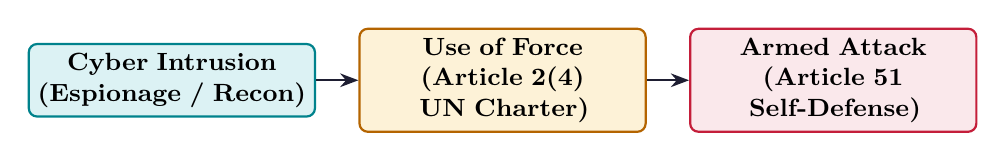
\begin{tikzpicture}[node distance=0.8cm and 1.2cm,
  n1/.style={rectangle, draw=myteal, fill=hdrteal, text width=3.4cm, align=center, minimum height=0.85cm, font=\small\bfseries, rounded corners=3pt, line width=0.8pt},
  n2/.style={rectangle, draw=myamber, fill=hdramber, text width=3.4cm, align=center, minimum height=0.85cm, font=\small\bfseries, rounded corners=3pt, line width=0.8pt},
  n3/.style={rectangle, draw=myred, fill=hdrred, text width=3.4cm, align=center, minimum height=0.85cm, font=\small\bfseries, rounded corners=3pt, line width=0.8pt},
  arrow/.style={-Stealth, thick, color=mydark}]

  \node[n1] (c1) at (0,0) {Cyber Intrusion\\(Espionage / Recon)};
  \node[n2] (c2) at (4.2,0) {Use of Force\\(Article 2(4) UN Charter)};
  \node[n3] (c3) at (8.4,0) {Armed Attack\\(Article 51 Self-Defense)};

  \draw[arrow] (c1) -- (c2);
  \draw[arrow] (c2) -- (c3);

\end{tikzpicture}
\end{tcolorbox}

\subsection{International Treaties and Frameworks}
\begin{itemize}[leftmargin=*, itemsep=4pt]
  \item \textbf{Tallinn Manual 2.0:} Non-binding study on applying international law to cyber operations, defining when a cyber attack constitutes an `Armed Attack` under Article 51 of UN Charter.
  \item \textbf{Budapest Convention on Cybercrime (2001):} International treaty standardizing national cybercrime legislation and enabling cross-border digital evidence sharing.
  \item \textbf{UN GGE Norms:} Voluntary non-binding norms prohibiting states from damaging each other's critical infrastructure during peacetime.
\end{itemize}

% ═══════════════════════════════════════════════════════════════════════════════
% QUICK REVISION PAGE
% ═══════════════════════════════════════════════════════════════════════════════
\newpage
\begin{center}
  {\large\bfseries\color{myred} Quick Revision --- Module 4}\\[3pt]
  {\small\color{mydark} Cyber Infrastructure Issues \& International Relations $|$ OE-EC803C}
\end{center}
\noindent{\color{myred}\rule{\linewidth}{1.2pt}}
\vspace{4pt}

\begin{tcolorbox}[formulabox, title={\textbf{Key Concepts and Metrics at a Glance}}]
\renewcommand{\arraystretch}{1.35}
\begin{tabularx}{\linewidth}{B{4.8cm} X}
SWIFT CSCF & Mandatory baseline controls for global banking messaging terminals. \\[3pt]
HIPAA Safeguards & Administrative, Physical, and Technical controls for patient health data. \\[3pt]
First-Party Insurance & Covers direct losses (forensics, downtime, ransomware payments). \\[3pt]
Third-Party Insurance & Covers customer lawsuits and regulatory non-compliance fines. \\[3pt]
Tallinn Manual 2.0 & International legal manual defining cyber warfare armed attack thresholds.
\end{tabularx}
\end{tcolorbox}

\begin{tcolorbox}[defbox, title={\textbf{One-Line Definitions}}]
\begin{itemize}[leftmargin=*, itemsep=2pt, topsep=0pt]
  \item \textbf{CNI:} Critical National Infrastructure vital for national security and public safety.
  \item \textbf{Systemic Risk:} Cascading failure across dependent entities from a single cyber event.
  \item \textbf{Budapest Convention:} International treaty facilitating cross-border cybercrime prosecution.
  \item \textbf{Article 51 UN Charter:} Inherent right of self-defense against armed cyber attacks.
\end{itemize}
\end{tcolorbox}

\begin{tcolorbox}[exambox, title={\textbf{Frequently Asked / Viva Questions}}]
\begin{enumerate}[leftmargin=*, label=\textbf{Q\arabic*.}, itemsep=5pt, topsep=0pt]
  \item \Q{Define Critical National Infrastructure (CNI).}
        Systems and networks so vital that their incapacitation would paralyze national security, economy, or public safety.

  \item \Q{Describe the Bangladesh Bank SWIFT heist of 2016.}
        Attackers used malware on local bank terminals to issue 35 fraudulent SWIFT requests, stealing \$81 Million.

  \item \Q{Explain the 3 HIPAA safeguard categories for healthcare security.}
        Administrative Safeguards (policies), Physical Safeguards (facility controls), and Technical Safeguards (AES-256 encryption, access control).

  \item \Q{What is the Tallinn Manual 2.0?}
        An authoritative study detailing how international law applies to cyber espionage, sovereignty, and state-sponsored cyber warfare.

  \item \Q{Distinguish between First-Party and Third-Party Cyber Insurance.}
        First-party covers direct operational costs (forensics, ransomware, downtime); Third-party covers customer lawsuits and regulatory fines.

  \item \Q{What is Systemic Risk in cyber insurance underwriting?}
        The risk that a single zero-day exploit or cloud outage cascades across thousands of insured companies simultaneously.

  \item \Q{What is the Budapest Convention on Cybercrime?}
        An international treaty harmonizing national cyber laws and facilitating cross-border digital evidence collection.

  \item \Q{How does Article 51 of the UN Charter apply to cyber attacks.}
        Allows a state to exercise military self-defense if a cyber attack causes physical destruction or human casualties equivalent to an armed attack.

  \item \Q{What are SWIFT CSCF mandatory controls?}
        Controls mandating network isolation of SWIFT terminals, strict MFA, and continuous transaction monitoring.

  \item \Q{What is Moral Hazard in cyber insurance?}
        The tendency of an insured firm to reduce its security spending, relying on insurance payouts to handle breaches.

  \item \Q{Explain the War Exclusion Clause in cyber insurance.}
        A clause allowing insurers to refuse payouts if a breach is attributed to a state-sponsored act of war.

  \item \Q{What is the role of UN GGE in cyber diplomacy?}
        Developing non-binding international norms prohibiting states from conducting malicious cyber attacks against critical civilian infrastructure.

  \item \Q{Why are connected medical devices (IoMT) vulnerable?}
        Because infusion pumps and MRI machines run unpatched embedded OSs, making them targetable by ransomware.

  \item \Q{Define Operational Technology (OT).}
        Hardware and software that detects or causes physical changes through direct monitoring of industrial plant equipment.

  \item \Q{What is the primary defense against SCADA air-gap bridging malware?}
        Strict USB port lockdown, disabling autorun, and scanning all external media before connecting to OT systems.
\end{enumerate}
\end{tcolorbox}

\begin{tcolorbox}[tikzbox, title={Summary Comparison: Infrastructure Security Requirements}]
\centering
{\renewcommand{\arraystretch}{1.45}%
\begin{tabularx}{\linewidth}{|B{3.0cm}|Y|Y|Y|}
\hline
\textbf{Infrastructure Sector} & \textbf{Regulatory Standard} & \textbf{Primary Security Control} & \textbf{Main Operational Concern} \\
\hline
Financial Banking & SWIFT CSCF / PCI-DSS & Hardware Security Modules (HSM) & Wire Fraud \& Account Takeover \\
\hline
Healthcare & HIPAA Security Rule & Field-Level AES Encryption & Ransomware \& Patient Safety \\
\hline
Energy Grid & NERC-CIP Standards & Purdue Level 3.5 Air Gap & Plant Sabotage \& Blackouts \\
\hline
Transportation & NIST SP 800-82 & Industrial Protocol Firewalls & Signaling Tampering \\
\hline
\end{tabularx}}
\end{tcolorbox}

\end{document}
